
\newpage
\section{Prototype Design}

\subsection{The Mobile Platform}

`Mobile phone adoption presents us with highly available, contextually aware and interactive platforms'~\cite{article_mhealth}.
Research into designing systems for mobile behaviour change technology, presents us with some implementation design requirements.
Implementing a prototype using these design considerations produces a solid ground for building this system.\newline
\newline

\subsection{Design Considerations}

Current mobile systems use apps to interact with users, but a recent study showed apps fall into a low behavioural theory adherence scale~\cite{article_mhealth}.
Research into how to build systems that are theory-based, suggest four main stages for designing mobile health solutions. Conceptualisation, Formative Research and Pretesting,
Pilot trials and Evaluation trials~\cite{article_mhealth}. The first two stages use the Behaviour Change Wheel~\cite{article_behaviour_change_wheel}
(a framework for planning health behaviour interventions), to understand the behaviour, better define the characteristics and form the mobile concept into a prototype.
The pilot trials tests the prototype before it moves to a finalised app with the commitment of a full trial. The final stage tests the finalised app with a wider range of participants.
This project will use these four stages as design steps to build the prototype.\newline
\newline

\subsection{Prototype Medium}

This section explores different mediums to develop a prototype, looking into if there is a better method to interact with users than a mobile app. Concludes with developing a Facebook Messenger Chatbot.\newline
\newline
When it comes to mobile phones, users have pleanty of options for interation. A popular choice that has revisited the market are Chatbots, applications that parse questions using Natural Language Processing (NLP) to provide a response, acting as a user interface to expose data. These programs have conversations with users to achieve a goal and are not new inventions. Since 1966~\cite{article_eliza}, Eliza by Joesphs Weizenbaum, used simple expression matching to return a certain response for user trials. In the present day, these applications (commonly referred to as bots, sometimes chatbots), are found integrated into many different apps on the majority of users mobile phones. For example, Facebook Messenger (a popular messaging application) encourages developers to create bots to interat with their users. These bots act as a real person with similar interaction flow, plus a few additional features, such as \textit{Quick Replies} for revealling a list of options to a user. `Quick Replies provide a way to present buttons to the user in response to a message.'~\cite{doc_fb_quick_replies}. However, these bots would not reply like a real person, but rather would only reply if that question was pre-trained using machine learning algorithms. This technology requires the bot to be trained on a large set of data and the majority of use cases would have to be accounted for.\newline
\newline
NLP would enable users to chat to the bot and get a friendly understandable reply. But, would this interaction develop a dependance on the user-chatbot interaction? Would it lead to losing atomaticity if the chabot supported habit formation? NLP will not be used to avoid these potential problems, and instead of natural language processing, the location of the bot (i.e. inside of an existing messaging app), ease of interaction and the additional features (quick replies) will help us easily communicate with a user.\newline
\newline
Another option is a website. But a website cannot send users reminders, unless it is paired with an app or SMS platform, but this is hard to get a reponse from a user.\newline
\newline
<table showing pros and cons of: Chabot, App, Cross-Platform app, Website>\newline

% \subsubsection*{Methods of implementation}
% `There are two main reasons why anyone would use a chatbot:
% Conversational: When an App can’t do it because multiple variable inputs are needed to solve the problem.
% Simplicity: When a bot offers the most immediate and direct solution to a person’s problem.'
% We are going to use the bot because what a bot offers directly solves our problems above.

% - 3 Types:
%   1. specific apps
%     - Bad cuz takes a long time
%   2. Web Apps
%     - Still another app
%   3. Chatbot
%     - Good useful
% - Android/iOS/chatbot specific notifications from web app
% - Save to home screen

% \subsubsection*{Technology}
% Talk about different chatbot tech available, e.g. amazon lex, and why im choosing fb messenger
% \url{https://aws.amazon.com/lex/}

% Web app could be chosen because its easiest and achievable, however the ease of use with a chatbot, integrated into fb messenger means everyone can use it on multiple devices. The addition, means that people get used to the UI.


\newline
Chatbot decided as best method to interact with lots of people easily, after table of pros and cons. Now the real question becomes, would users be able to develop habits with a conversational user interface. Disucssion about other types of chatbots, e.g. SMS bot, or Slack bot.

% TODO insert photo of another type of chatbot, e.g. slack bot and SMS bot

Facebook Messenger looks like an attractive option for user interaction:

- Installed on the top 90\% of peoples phones
- Embeded into a service users already use
- Quick replies allows for easy interaction

But, will users differentiate between a bot and a person? Will the text interaction put people off? This thesis aims to answer those questions.

\subsection{Facebook Messenger}

\begin{figure}[ht] % ht
    \centering
    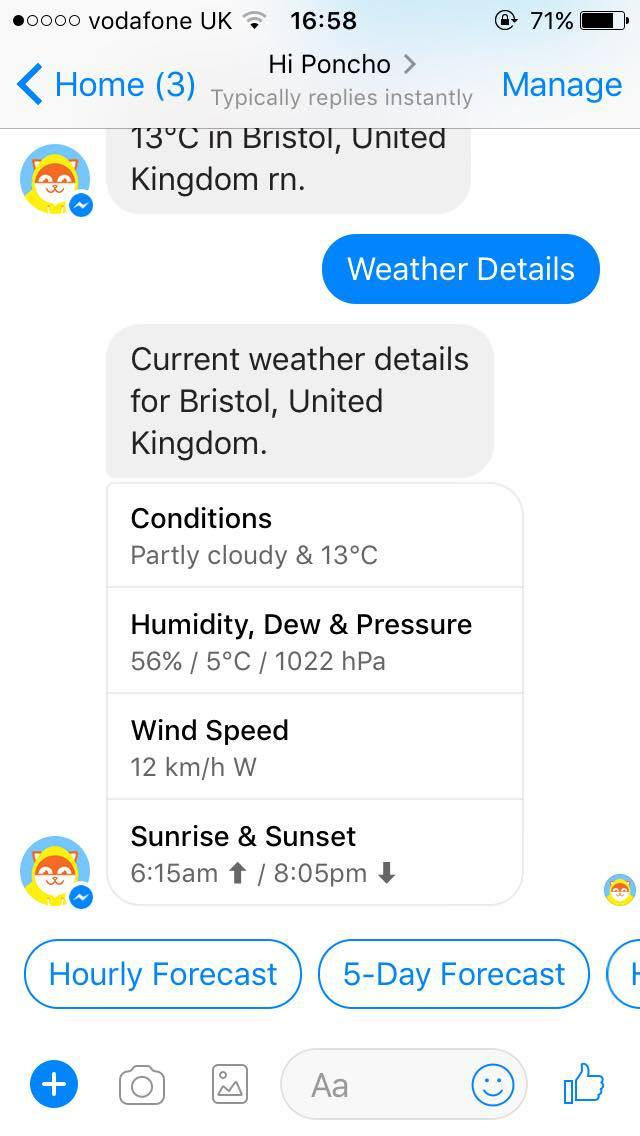
\includegraphics[width=2.5in]{../resources/poncho.jpg}
    \caption{Poncho: An example of Facebook Messenger Weather Chatbot}
    \label{fig:poncho}
\end{figure}

Discussion about the additonal features fb messenger has with discussion about previuos chatbots.

<photo of UI flow>

<photo of quick replies>

\begin{figure}[ht]
  \centering
  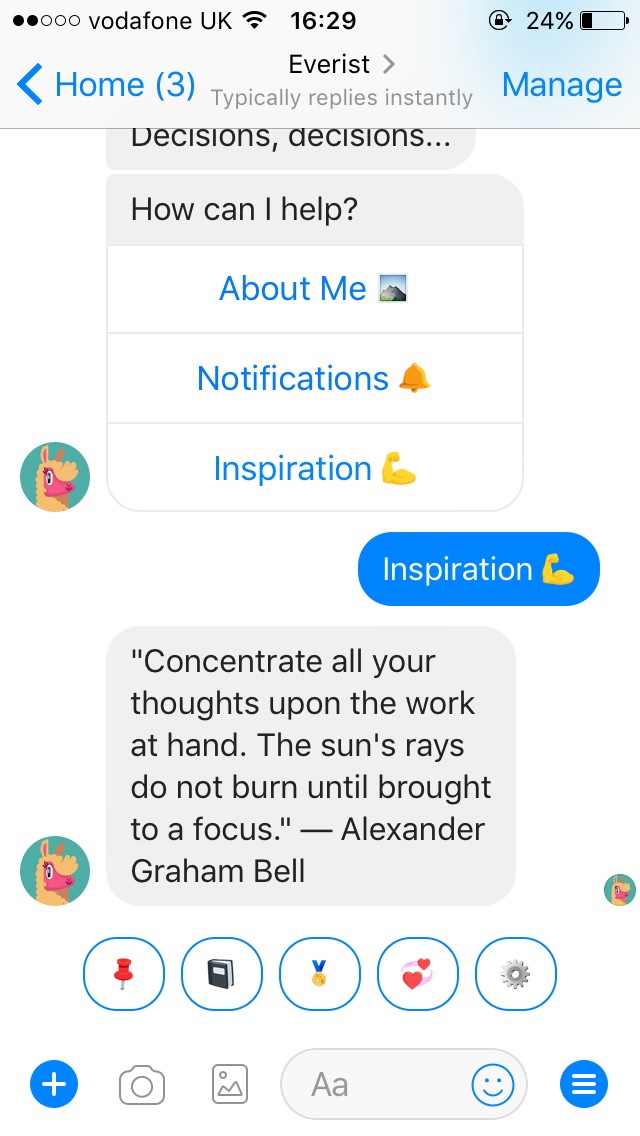
\includegraphics[width=1.9in]{../resources/everist.png}
  \hspace{10px}
  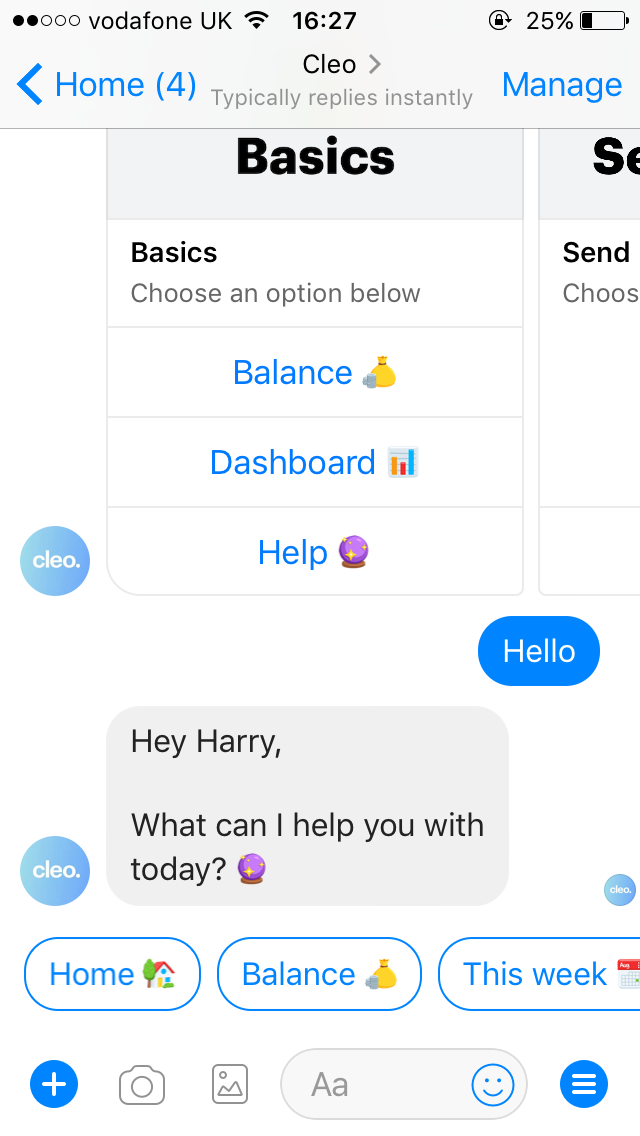
\includegraphics[width=1.9in]{../resources/cleo.png}
  \hspace{10px}
  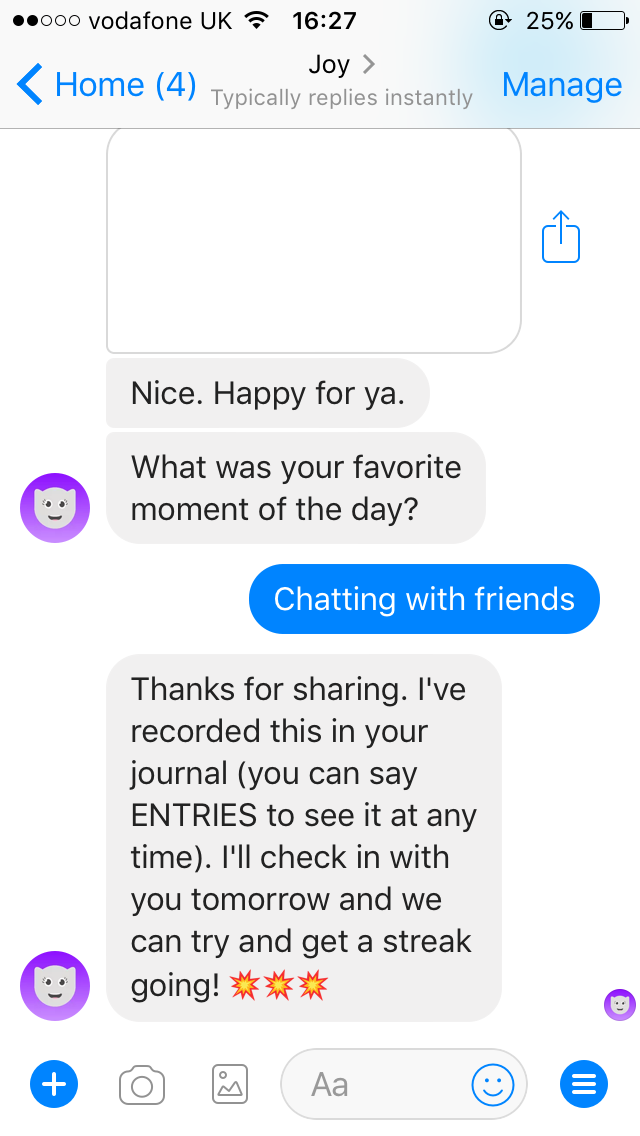
\includegraphics[width=1.9in]{../resources/joy-ai.png}
  \caption{Examples of chabots performing different actions}
  \label{fig:chatbots_examples}
\end{figure}


\subsection{Supporting Habit Formation}

Discussion about how we can support habit formation using a chatbot in realaity.

% \subsection*{Gamification Elements}
% - Gamification elements~\cite{article_free_to_play_making_money_from_games_you_give_away}
% - Designing outstanding feedback loops~\cite{website_how_to_design_feedback_loops}


\subsection{Delivering Rewards}

Discussion about how the rewards will be delivered to the users. Inline verses same screen. How interaction is hanlded. Concludes with exaclty how rewards will be handled in design way, breif discussion about vibration and how it would not work.

<photo of inline verses non-inline>

The types of rewards are separated into three categories, visual, auditory and combined visual-auditory. Different types of these rewards will be experiemented with,
and test if they provide user satisfaction. These rewards will be displayed to the user within the chatbot after they complete their habit.
For a playful prototype, visual rewards will be light-hearted gifs and auditory rewards will be selected to match the gifs.


% - Vision
%   - Send notification
%   - Show nice visuals

% - Audio
%   - Send notification
%   - Play uplifting music

% - Tactile Vibration
%   - A.P.I. sets wearable alarm
%   - Wearable (fitbit) issues and tracks alarm times


\subsection{User Flow}

Full user interaction from setup to completing a reward.

%   - Setup:
%     - Setup the bot via a messaging platform, such as fb messenger
%   - Trigger:
%       - Either A, certain configured time of the day
%       -        B: No trigger
%       -        C: Around a specific time
%   - Action:
%     - Choose habit from list of habits
%     - Perform
%     - Use app to track the action
%   - Reward:
%     - You get one of these rewards, based on modalitiy selected
%     - Vision
%       - Through message, of an image or gif
%       - Could be: App, or message, gif
%     - Audatory
%       - Through phone via bot, link to mp3/spotify/apple music
%       - Could be: App
%     - Tactic
%       - Through wearable
%       - Could be: App, bot triggers wearbale alarm


% \subsection{User Flow}
%   - Pre-Start
%     - Choose daily habit type from list of X, e.g. 1 press up before breakfast
%     - Enable notifications or fitbit if chosen
%     - Time action / reward, variable rewards, e.g. then work out average time to send, or none
%   - Start:
%     - New day
%     - @ trigger time, send reminder, if set, notification
%     - Open notification, do habit, press tracked
%     - Get reward type


\section{Prototype Implementation}

Abstract implementation overview of user and chatbot discussion.

<photo sketched>
%   % [app] -------> (Database) -----> at certain time ---> Send notification to trigger type of reward
%   % [ big button that says track]
%   % taskname textbox

% Flow diagram style
% \tikzstyle{startstop} = [rectangle, rounded corners, minimum width=3cm, minimum height=1cm,text centered, draw=black, fill=red!30]
% \tikzstyle{io} = [trapezium, trapezium left angle=70, trapezium right angle=110, minimum width=3cm, minimum height=1cm, text centered, draw=black, fill=blue!30]
% \tikzstyle{process} = [rectangle, minimum width=3cm, minimum height=1cm, text centered, draw=black, fill=orange!30]
% \tikzstyle{decision} = [diamond, minimum width=3cm, minimum height=1cm, text centered, draw=black, fill=green!30]
% \tikzstyle{arrow} = [thick,->,>=stealth]

% \begin{tikzpicture}[node distance=2cm]
%   \node (user) [startstop] {User};
%   \node (fbmsgr) [process, below of=user] {Messenger};
%   \node (chatbot) [process, below of=fbmsgr] {Chatbot};
%   \node (responses) [process, right of=chatbot, xshift=4cm] {Responses};
%   \node (userend) [startstop, below of=chatbot] {User};

%   \draw [arrow] (user) -- node[anchor=east] {Opens} (fbmsgr);
%   \draw [arrow] (fbmsgr) -- node[anchor=east] {Message} (chatbot);
%   \draw [arrow] (chatbot) -- node[anchor=south] {Message} (responses);
%   \draw [arrow] (responses) -- node[anchor=north] {Response} (chatbot);
%   \draw [arrow] (chatbot) -- node[anchor=east] {Notification} (userend);
% \end{tikzpicture}

\subsection{Platform}

Language consideration, nodejs, java, other types, talk about heroku, hosting provider. Hosting provider.
Database provider discussion, integration, airtable,

\subsection{Reward Limitations}
Breifly Vibration limitations

\subsection{Detailed Overview}

Architecture Component overview w diagram
Chatbot function overview w diagram
Implementation limitations
Scheduler
Free text input

\newpage
